\section{基于P2P网络的信息自主流动机制的研究}
本章将基于上一章提出的用户兴趣模型给出建立用户兴趣覆盖网络的基本思路和方法。首先,从宏观上给出整个网络的组织架构和拓扑结构,由于是非中心化的P2P,因此网络中的每个节点既要充当服务端也可以作为客户端,如何能够快速发现兴趣相同的节点在信息传播中是尤为重要的。然后,从微观上来看,每个节点存储的信息是决定整个网络流动是否顺畅的基础,因此本章将充分利用用户兴趣集的特性来构建节点存储结构,并阐述如何利用该结构快速找到潜在的目标节点。

\subsection{用户兴趣覆盖网络的构建}
在第二章中提到了用户之间遵循一种关注-被关注的关系,这在社交网络中是十分常见的,因此这里直接将这种关系引入,默认用户节点直接会实现存储一些时常关注的邻居节点。整个网络的架构如图\ref{fig:overlay}所示,图(A)是节点初步连接后的结果。可以看到,在用户关注关系层上,用户$u_1$和用户$u_3$并没有直接的关注或被关注的关系,$u_3$必须先后间接通过$u_4$和$u_3$才能连接到。但是在上面的用户兴趣关系层中,用户$u_1$和$u_3$之间直接建立了关系,依据是他们拥有共同的兴趣(图中绿色边表示)。此时,用户$u_1$充当的是服务器,他将自己的资源1和资源2分别传播给了另外三个用户,并且转播的依据是存在共同兴趣。当经过一系列运作以后,用户兴趣关系层中的拓扑结构会发生变化,如图(B)所示。可以看到,用户$u_4$和$u_1$、$u_2$之间发现了新的兴趣(图中蓝色边表示)。此时,用户$u_4$作为信息发布者将资源3传播给这两个节点,因此$u_1$此时充当了资源接受者,但同时$u_1$也在继续发布资源1,它充当了两个角色。这就是基于P2P网络的一个实例,在构建这样一个覆盖网络归结起来要解决这样两个问题:
\begin{itemize}
  \item 节点的数据存储结构:因为整个网络是一个非结构化的拓扑,也就是说没有中心服务器来直接获得其他节点的信息。所以,每个节点必须自己存储其他部分节点的信息。
  \item 节点间兴趣导向边的建立:节点与节点之间的关系在用户兴趣关系层上表现为两个用户具有共同的兴趣。以上一章的用户兴趣模型来看,也就等价于两者的兴趣集中存在公共兴趣点集合。
\end{itemize}

\begin{figure}[!ht]
\centering
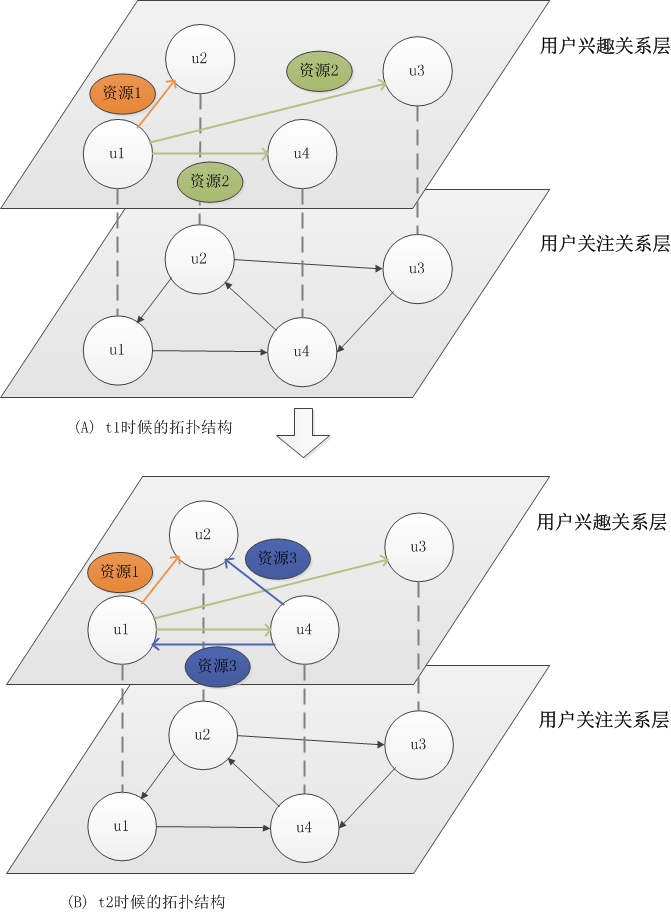
\includegraphics[width=\textwidth]{overlay.png}
\caption{基于P2P的兴趣覆盖网络示意图}
\label{fig:overlay}
\end{figure}

\subsubsection{节点的数据存储结构}
在基于P2P的兴趣覆盖网络中,几乎所有节点都会既要充当信息发布者,又要充当信息接受者,既同时作为服务器和客户端。考虑到这种网络的特性,需要给节点加入以下一些松耦合的规则才能形成。虽然最终得到的拓扑结构具有一定属性,但数据项的设计不能像结构化拓扑中的那样基于任何拓扑相关的知识。在之后的搜索过程中,先要找到一个数据项,查询该节点其邻居,最典型的查询方法是泛洪。该查询协议是对一定范围内的所有的邻居进行搜索,因此需要在物理上存储周围这些节点的信息。这样的设计是非常有弹性的,特别是对于那些进入和离开该系统的节点。

因此,每个节点的需要保存的数据结构如图\ref{fig:data}所示:
\begin{figure}[!ht]
\centering
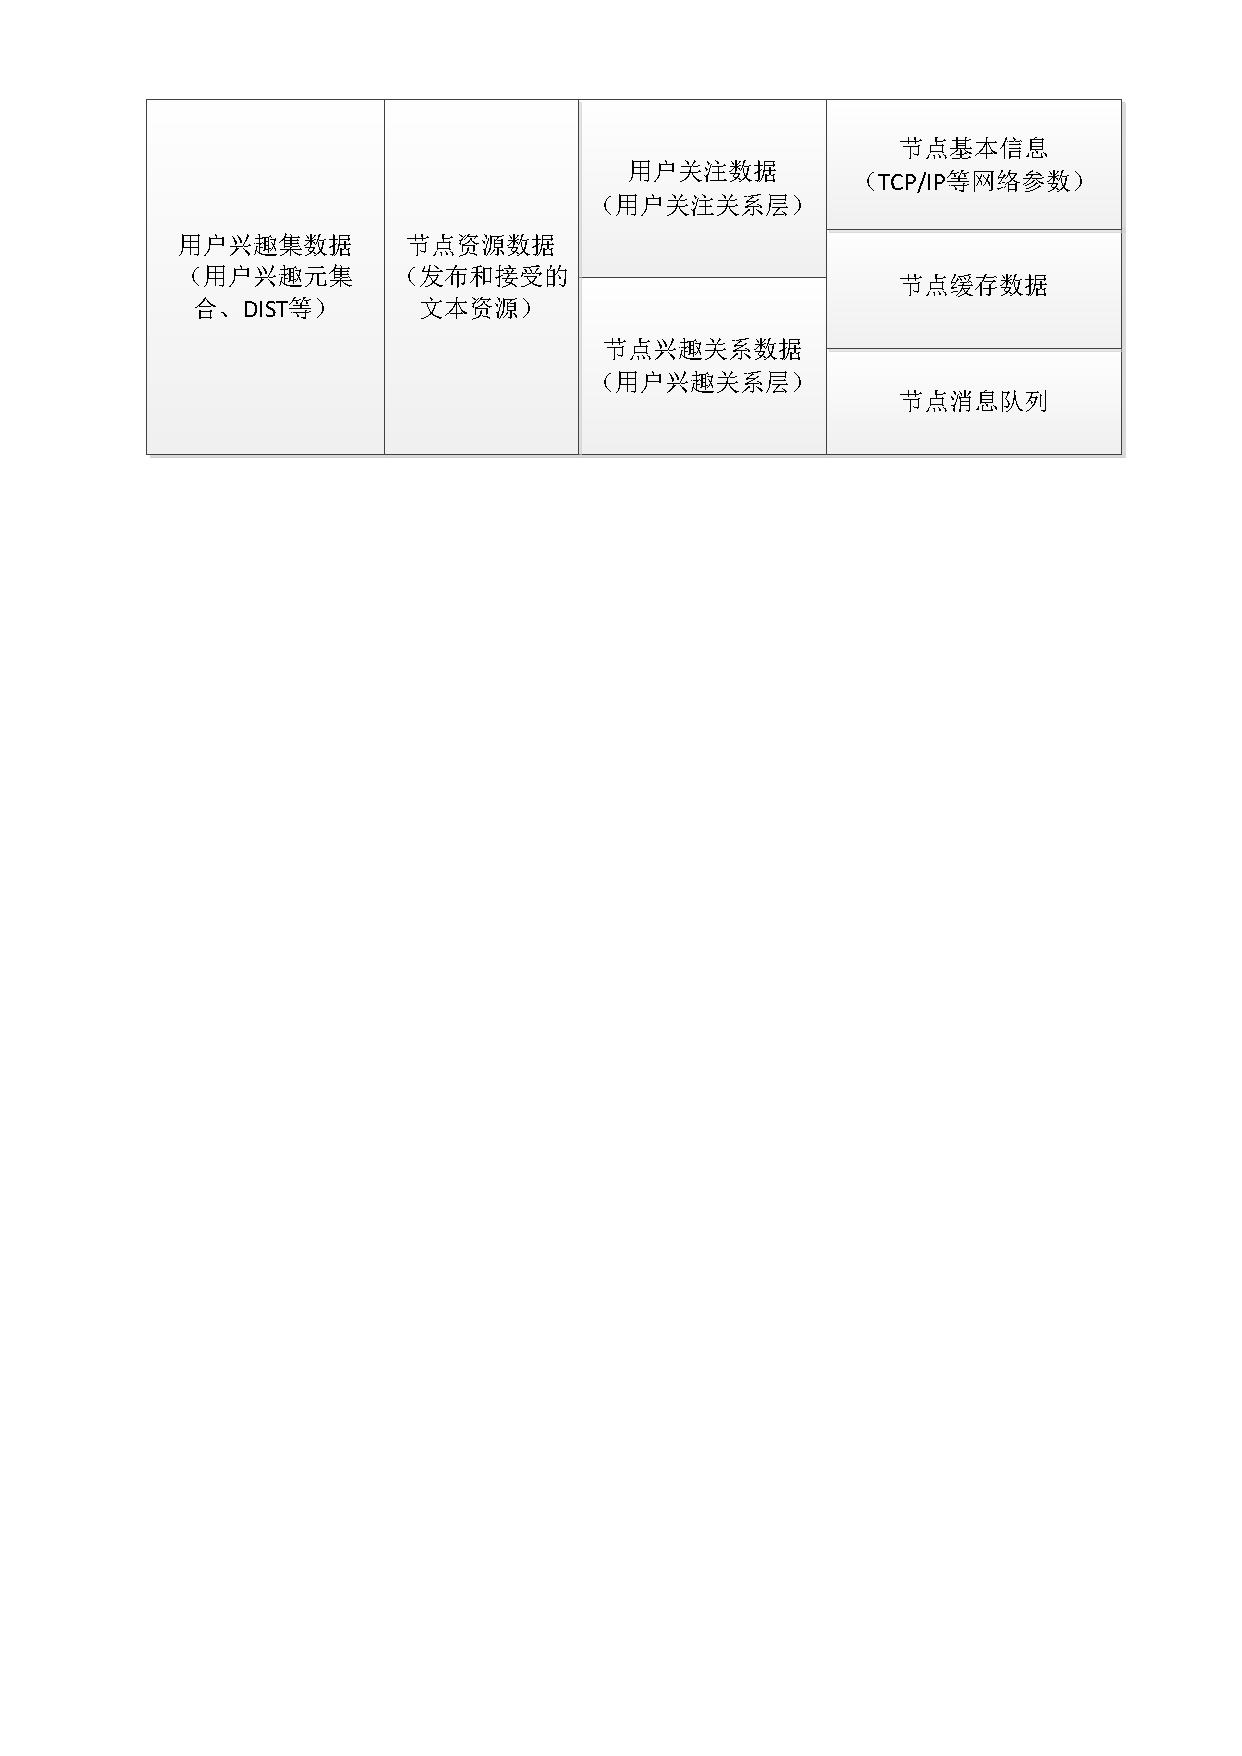
\includegraphics[width=\textwidth]{data.pdf}
\caption{兴趣覆盖网络中节点的数据结构}
\label{fig:data}
\end{figure}

\begin{enumerate}
  \item 节点基本信息:节点在TCP/IP上的基本信息,包括IP地址、节点ID等,这些信息用来方便其他节点进行定位。换句话说,当节点之间要直接通信时,可以根据这些数据直接连接,这里的通信仍然遵循物理网络中的协议。
  \item 用户关注数据:这里存储的是用户关注关系层中的数据,即用户关注的其他用户节点列表,列表中的信息包括上述基本信息,主要是在网络初始化的时候,节点用来寻找其他潜在的兴趣相同的节点。
  \item 用户兴趣集数据:这里的用户兴趣集和上文中提出的概念是一致的,具体参见第四章相关的讨论。
  \item 节点兴趣关系数据:这里存储的是用户兴趣关系层中的数据,包括具有共同兴趣的用户节点信息,共同兴趣集的数据等。
  \item 节点资源数据:当用户生成新的文本资源时,资源副本都会在本地进行保存。同理,用户接受的文本资源也会进行存储。此外,该部分数据还包括了用户对收到资源的反馈、关联的发布者信息、其他节点收到资源后反馈的信息等等。
  \item 节点消息队列:缓存中需要发送和接受的消息,包括节点的基本信息,兴趣集等。
  \item 节点缓存数据:在网络通信中临时保存的数据,这些数据主要用于方便其他节点更加快速地找到资源,以及方便自己找到其他兴趣类似的节点。
\end{enumerate}

\subsubsection{兴趣覆盖网络的初始化过程}
这部分的工作是为了在用户兴趣关系层中建立节点之间的边,这里的边称为兴趣导向边。换句话,一旦两个节点之间有边相连时,说明两个用户之间存在较为明显的共同兴趣,关于如何根据用户兴趣集求出共同兴趣点集合的算法参见第四章。如图\ref{fig:initoverlay}所示,下面对兴趣覆盖网络的初化化过程进行说明:

\begin{figure}[!ht]
\centering
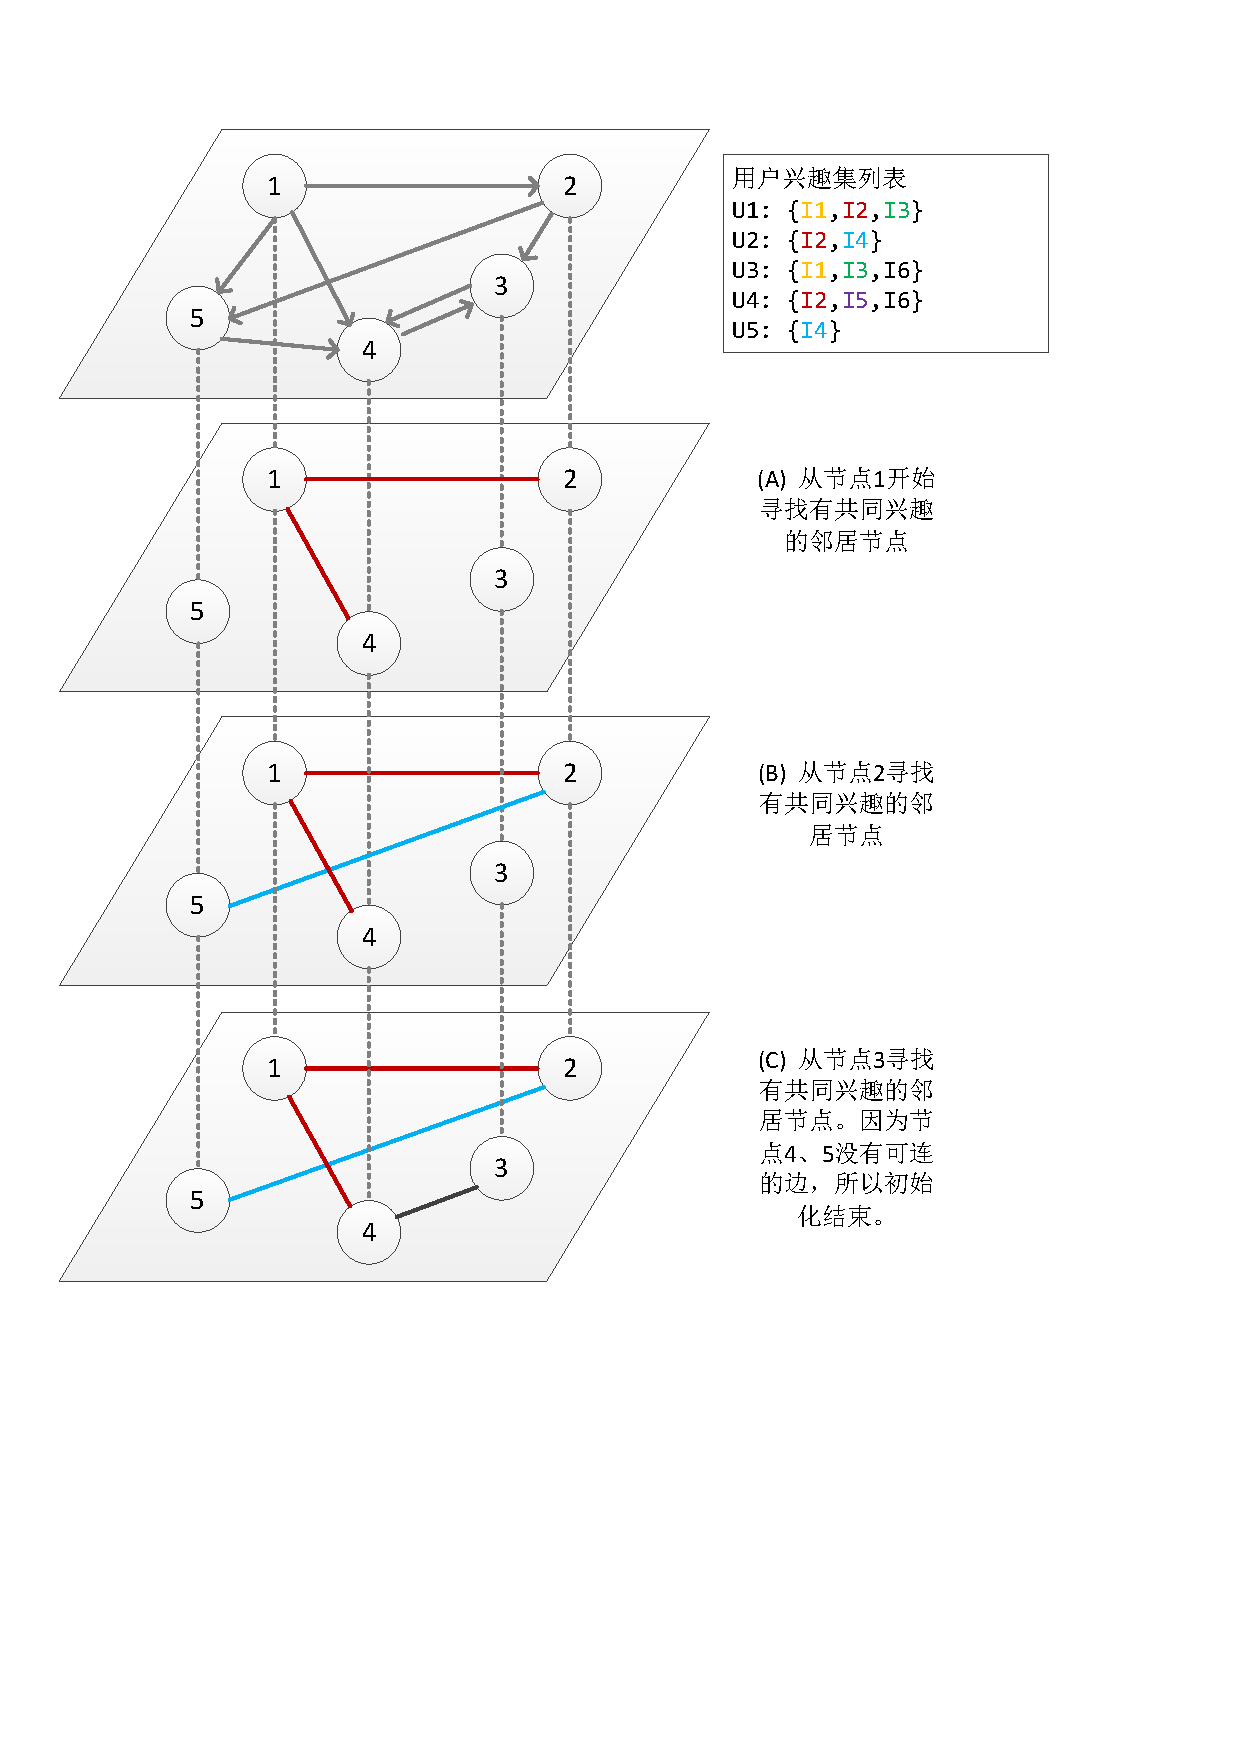
\includegraphics[width=\textwidth]{initoverlay.pdf}
\caption{兴趣覆盖网络的初始化实例}
\label{fig:initoverlay}
\end{figure}

在整个初始化过程中,我们使用Iterative Deepening的方式进行路由,为了简化问题,这里设置TTL=1,即在网络中只执行一跳。
\begin{enumerate}
  \item 如图(A)所示,先从节点1开始寻找具有相同兴趣的邻居节点。从用户关注关系层中可以发现,节点1关注了节点2、4、5,因此依次访问这三个节点进行判断。这里共同兴趣的判断采用了简化的模式,即认为两个兴趣集的交集元素是共同元素(实际判断方法还要引入DIST和SICT进行相似度的计算)。经过计算后发现,节点1和节点2有共同兴趣$I_2$,与节点4也有共同兴趣$I_2$,所以在用户兴趣关系层中这这三个节点间分别建立兴趣导向边(图中红色的边)。
  \item 如图(B)所示,节点2继续寻找具有相同兴趣的邻居节点。从用户关注关系层中发现,节点2关注了节点3、5,因此依次访问这两个节点来判断是否有共同兴趣。经过计算后发现,只有节点2和节点5之间存在共同兴趣$I_4$,因此建立一条兴趣导向边(图中蓝色的边)。
  \item 如图(C)所示,节点3继续寻找具有相同兴趣的邻居节点。从用户关注关系层中发现,节点3关注了节点4,经过计算后判断出它们之间有共同兴趣$I_6$,从而建立一条兴趣导向边(图中黑色的边)。对节点4和节点5执行相同的操作,发现它们与其他的节点之间都没有可以新增的兴趣导向边,所以初始化结束。
\end{enumerate}

从上述例子中可以总结出以下几点。第一,虽然在用户关注关系层中边的数量比较多,但是在最后的用户兴趣关系层中边的数量却要少很多。导致这个现象的原因可能是因为这些节点间共同的兴趣集十分少,用户之间之所以关注是因为社交网络中好友的关系。第二,在用户兴趣关系层中,每个节点拥有的边的数量也减少很多,这样的好处是用户只会接受到兴趣相似的用户发来的资源,从而可以过滤掉没用的信息。第三,这里设置的TTL为1,因此在用户兴趣关系层中的边数比较少,但是如果将TTL设置更大一下,本来没有相互关注的节点也会直接建立兴趣上的连接。

\subsection{兴趣覆盖网络拓扑结构的更新}
根据第四章中关于用户兴趣讨论的内容可知,动态性是用户兴趣的主要特征之一,而且在实际应用中十分重要。因此当用户兴趣发生变化时,用户兴趣关系层中的拓扑结构也会发生相应的变化,如图\ref{fig:updateoverlay}所示为用户产生新兴趣时结构变化的过程。

\begin{figure}[!ht]
\centering
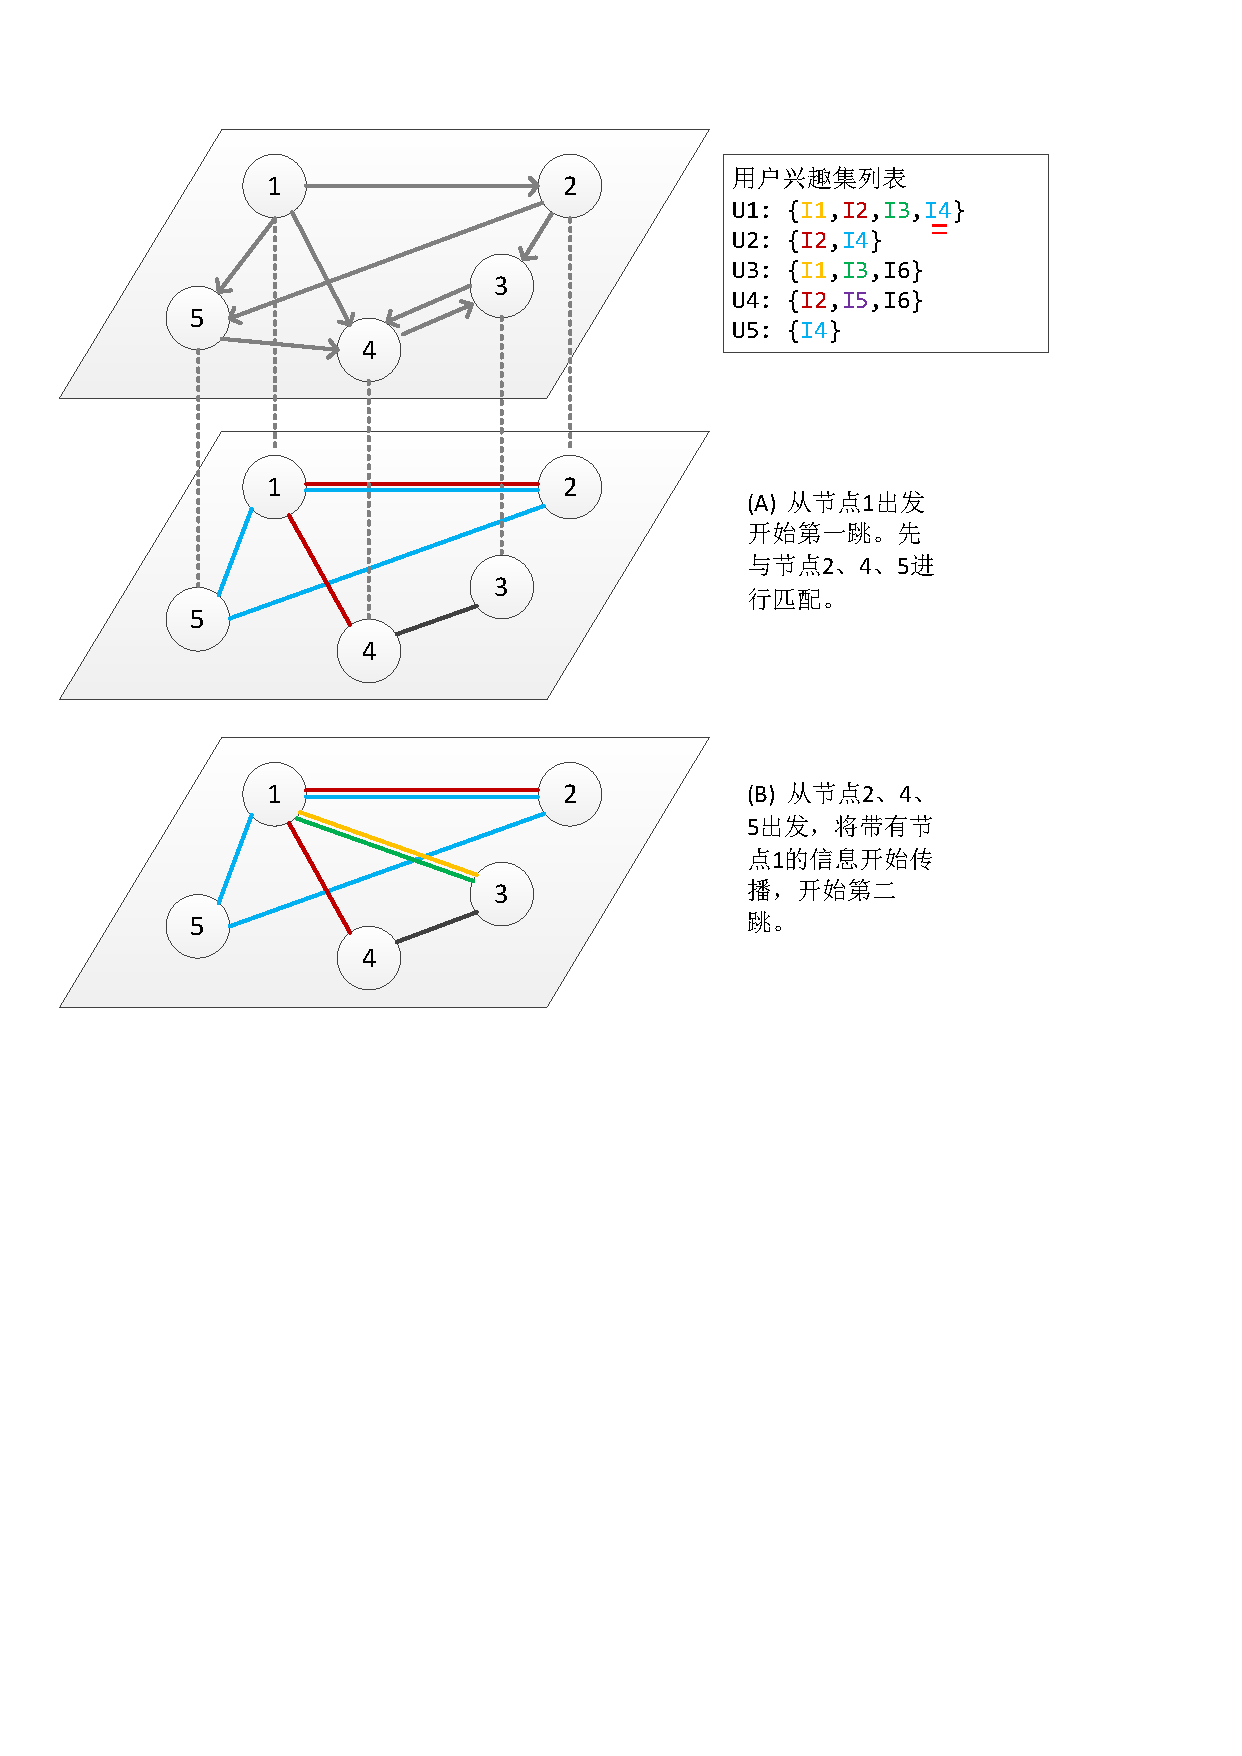
\includegraphics[width=\textwidth]{updateoverlay.pdf}
\caption{当用户兴趣变化时,兴趣覆盖网络拓扑调整的实例}
\label{fig:updateoverlay}
\end{figure}

\begin{enumerate}
  \item 如图(A)所示
\end{enumerate}

\subsection{兴趣覆盖网络的资源传播}
//todo

\subsection{小结}
//todo
